\documentclass[conference]{IEEEtran}
\IEEEoverridecommandlockouts
% The preceding line is only needed to identify funding in the first footnote. If that is unneeded, please comment it out.
\usepackage{cite}
\usepackage{amsmath,amssymb,amsfonts}
\usepackage{algorithmic}
\usepackage{graphicx}
\usepackage{textcomp}
\usepackage{xcolor}
\usepackage{float}
\usepackage{caption}
\usepackage{booktabs}
\usepackage{tabularx}
\usepackage{subcaption}
\usepackage{adjustbox}
\usepackage{url}

\def\BibTeX{{\rm B\kern-.05em{\sc i\kern-.025em b}\kern-.08em
    T\kern-.1667em\lower.7ex\hbox{E}\kern-.125emX}}

%\addbibresource{../book/misc/bibliography.bib}


\begin{document}

\title{YOLOv911: An Improvement to YOLOv7 for Airborne Object Detection Task\\ 
%{\footnotesize \textsuperscript{*}Note: Sub-titles are not captured in Xplore and
%should not be used}
%\thanks{Identify applicable funding agency here. If none, delete this.}
}

\author{
    Dion Andreas Solang, Reza Fuad Rachmadi, I Ketut Eddy Purnama\\
    Department of Computer Engineering\\
    Faculty of Intelligent Electrical and Information Technology\\
    Institut Teknologi Sepuluh Nopember (ITS)\\
}


%\author{\IEEEauthorblockN{1\textsuperscript{st} Given Name Surname}
%\IEEEauthorblockA{\textit{dept. name of organization (of Aff.)} \\
%\textit{name of organization (of Aff.)}\\
%City, Country \\
%email address or ORCID}
%\and
%\IEEEauthorblockN{2\textsuperscript{nd} Given Name Surname}
%\IEEEauthorblockA{\textit{dept. name of organization (of Aff.)} \\
%\textit{name of organization (of Aff.)}\\
%City, Country \\
%email address or ORCID}
%\and
%\IEEEauthorblockN{3\textsuperscript{rd} Given Name Surname}
%\IEEEauthorblockA{\textit{dept. name of organization (of Aff.)} \\
%\textit{name of organization (of Aff.)}\\
%City, Country \\
%email address or ORCID}
%\and
%\IEEEauthorblockN{4\textsuperscript{th} Given Name Surname}
%\IEEEauthorblockA{\textit{dept. name of organization (of Aff.)} \\
%\textit{name of organization (of Aff.)}\\
%City, Country \\
%email address or ORCID}
%\and
%\IEEEauthorblockN{5\textsuperscript{th} Given Name Surname}
%\IEEEauthorblockA{\textit{dept. name of organization (of Aff.)} \\
%\textit{name of organization (of Aff.)}\\
%City, Country \\
%email address or ORCID}
%\and
%\IEEEauthorblockN{6\textsuperscript{th} Given Name Surname}
%\IEEEauthorblockA{\textit{dept. name of organization (of Aff.)} \\
%\textit{name of organization (of Aff.)}\\
%City, Country \\
%email address or ORCID}
%}

\maketitle
\thispagestyle{plain}
\pagestyle{plain}

\begin{abstract}    
%In this research, we present some approach to improve the capability of YOLOv7
%to detect airborne objects. Airborne objects appear very small on cameras due
%to their usually large distance to the camera. For that reason, YOLOv7 needs to
%be optimized to detect small objects. Several modification proposals was made and
%tested in this research. The modifications include changes in the architecture
%(adding extra detection layer, modifying feature-map source of the neck,
%and replacing detection head to a detached anchor-free head) and in Bag-of-Freebies
%(anchor recalculation and mosaic augmentation). We found the combination of
%mosaic augmentation, anchor recalculation, and modification of feature-map source of
%the neck produces a model with mAP 14.09\%, a significant improvement compared
%to plain YOLOv7 that produces mAP of 0\%.
%This document is a model and instructions for \LaTeX.
%This and the IEEEtran.cls file define the components of your paper [title, text, heads, etc.]. *CRITICAL: Do Not Use Symbols, Special Characters, Footnotes, 
%or Math in Paper Title or Abstract.
  In this research, we present some approach to improve the detection capability of YOLOv7 for airborne objects. 
  Airborne objects appear very small in camera images when they are located at a considerable distance from the camera. 
  However, due to their high speed of movement, it is crucial to detect them while they are still far away. 
  Therefore, to effectively detect these objects with YOLOv7, its small object detection capability must be enhanced.
  To address this challenge, we proposed several modifications that include changes in the architecture (adding an extra detection head, modifying the feature-map source, and replacing the detection head with a detached anchor-free head), application of bag-of-freebies techniques (anchor recalculation and mosaic augmentation), and change in the inference process (partitioning the image and performing inference on each partition).
  Through comprehensive experimentation, we have discovered that the combination of replacing the detection head with a detached anchor-free head, and performing inference on partitions yields the most promising results, with a significant increase in mean average precision (mAP) of 46.18\% while still maintaining real-time inference speed (greater than 10 FPS).
  This improvement is notably higher compared to the unmodified plain YOLOv7, which achieved an mAP score of 0\%.

\end{abstract}

\begin{IEEEkeywords}
Small Object Detection, YOLOv7, Architecture Modification, Bag-of-Freebies Modification, Airborne Object
\end{IEEEkeywords}

\section{Introduction}

Autonomous Aerial Vehicle (AAV) has the potential to significantly impact industries, particularly in commercial delivery \cite{prime_air}.
To realize this potential, a reliable and efficient Sense and Avoid (SAA) system is needed.
While the airspace in which AAVs operate may be relatively sparse, there are still risks of encountering static obstacles or airborne objects such as birds or other drones.
With an effective SAA system, we can mitigate these risks and safeguard both the AAV and the valuable cargo it carries during commercial delivery.

As most AAV uses camera as its sensor due to its smaller weight and lower price, 
there is a need for camera based object detection system for SAA purpose.
One problem is that, airborne objects can appear unexpectedly and approach rapidly from
long distances. For this reason, airborne objects must be detected as early as possible, which means
that they must be detected when their image on the camera were still very small. 
Thus, the object detector for SAA system must be able to detect small objects.

In this research, we attempt to optimize YOLOv7 to be able to perform airborne
object detection. YOLOv7 was chosen due to its ability to perform real-time
object detection accurately even under complex outdoor environment. 
At the time of execution of this research, YOLOv7 had the highest mAP score amongst all published real-time object detector \cite{yolov7}.
This research is not about finding the ultimate solution for airborne object detection, but rather an exploration of methods that can be used
to enhance YOLOv7 on detecting small objects, which extends to airborne objects.

To optimize YOLOv7, we defined a set of modification to be applied to YOLOv7
that includes modification to its neural network architecture, some applications
of bag-of-freebies, and modification on the way the neural network perform inference. 
To find the best probably optimal solution, we will try combinations of the modification within the set, and choose the one with the highest mAP score.

We will be using The Airborne Object Tracking (AOT) Dataset \cite{aot_dataset} to train
and test the modification combinations. AOT Dataset consist of aerial vehicle flights
footage. In this dataset, the resolution of each image are $2048\times2448$ px, meanwhile
the size of the airborne object bounding box can be as small as 4 px (0.00008\% of resolution).
An example of the dataset can be seen on Fig. \ref{fig:airborne-example}.

\begin{figure}[t]
\centerline{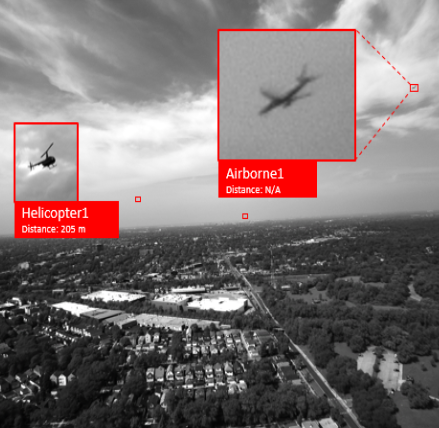
\includegraphics[width=0.45\textwidth]{../book/figures/dataset-example-labeled.png}}
\caption{Example Image from AOT Dataset (From \cite{aot_dataset})}
\label{fig:airborne-example}
\end{figure}

\section{Related Works}
Several attempts have been made in the past to increase YOLO architecture ability
to detect small objects. Here we present some of them.
\subsection{YOLO-Z}
YOLO-Z is a modification of YOLOv5 to optimize its ability to detect
cone for autonomous racing purpose \cite{yoloz}.
YOLO-Z modify the backbone of YOLOv5r5.0 to down-scaled DenseNet, while
the neck was changed to PANet.
These modification results in an increase of accuracy to detect cone
that are far away while still being able to do detection in real-time.
\subsection{exYOLO}
exYOLO used YOLOv3 as the basis for modification \cite{exyolo}. 
exYOLO modified
the neck of YOLOv3 by adding Receptive Field Block before combining the feature maps.
These modifications produce a higher mAP score than plain YOLOv3 on
PASCAL VOC2007 dataset.

\subsection{Barunastra ITS' Object Detection System 2022}
%TODO:this section
In \cite{barunastra}, a variant of YOLOv4-tiny was applied for the object detection system in
an Autonomous Surface Vehicle. This variant of YOLOv4-tiny added an additional detection layer
to the architecture, making the originally 2-head architecture of YOLOv4 tiny become 3-head.
This change in the architecture improved the detection capability, especially for small object, without
sacrificing latency too much.


\section{Experimental Setup}

\subsection{Computational Resource and Basis Model}
\label{section:instruments}
To conduct the experiment, we utilized Nvidia RTX 2080 Ti GPU which has 11 GB of VRAM.
We performed a pilot test with this hardware and found that
with this limited amount of memory, training large YOLOv7 model such as W6, E6, and E2E
is infeasible. Thus, we chose normal YOLOv7 with input size of 1600 and training batch-size of 1 as the basis model
for modification as it was the model with the largest input size that can be trained with enough free space in the 11 GB VRAM for minor architectural modifications.% and has a large input size.

%Not to add the large input size of the image. For this reason,
%the architecture that is chosen as the baseline for modification is the normal  size
%YOLOv7. The model will be trained with input size of $1600\times1600$ with batch size 1.

%Furthermore, the dataset that will be used to train the model will be limited to 400 images.
%The sampling strategy for the dataset will be explained in section \ref{section:dataset}.
%In a pilot test of the experiment, we found that to train a model for 300 epochs with 400 images
%with this setup, it will take around 20 hours. This is the reason why we limit the 
%amount of images to 400 and epoch to 300.
\subsection{Dataset}
\label{section:dataset}
The AOT dataset, consist of more than 11 TB images of drone camera footage.
Amongst these 11 TB of data, there are images taken from planned and unplanned encounters with
airborne objects. In this research, we sample the data from planned encounters.
There are millions of image in the planned encounters. To obtain 400 images
for training as explained in section \ref{section:instruments}
and some more for validation and testing, we use the sampling strategy
described in Table \ref{tbl:datasetsamplingdist}.

\begin{table}[htbp]
  \centering
  \caption{Dataset Sampling Strategy}
  \label{tbl:datasetsamplingdist}
  %\resizebox{\columnwidth}{!}{%
  \tabcolsep4pt
  
\begin{tabular}{c c c c c c c}
  \toprule[1.5pt]
  Splits    &Total &\multicolumn{5}{c}{Classes Percentage}\\
%                    \cline{3-7}
            &Images& Airplane & Helicopter & Bird & Drone & Negative\\
  \midrule
  Training  &400   &23.75\%   &23.75\%     &23.75\% &23.75\%       &5\%\\
  \midrule
  Validation&100   &20\%      &20\%        &20\%    &20\%          &20\%\\
  \midrule
  Test      &200   &20\%      &20\%        &20\%    &20\%          &20\%\\
  \bottomrule[1.5pt]
\end{tabular}
\end{table}

\subsection{Training Setup and Model Selection}
To train the YOLOv7 modified according to modification candidates in \ref{section:modifications},
we used images sampled as explained in \ref{section:dataset}. Each modification  was trained with 300 epochs at batch-size 1.
For validation, the experiment was repeated with a resampled data thrice, and have the average reported.

We define the best model as the model with the highest mAP@50 score.
However, to preserve the real-time capability of the selected model, models that will be considered
are only the model that can perform inference with speed more than 10 FPS.

mAP@50 was chosen instead of mAP@50:95 because we don't expect for the neural network to have a tightly fit bounding box prediction.
We consider a loose 50\% IoU coverage as good enough for a detection.

\subsection{Modifications}
\label{section:modifications}
Here we present the proposed modification candidates for YOLOv7

\subsubsection{Mosaic Augmentation}
Mosaic Augmentation was reported to increase the mAP score of the model in
\cite{yolov4}{yolov5}. This augmentation is simple to implement. Therefore,
we included mosaic augmentation in our set of modifications combine.

\subsubsection{Anchor Recalculation}
Anchor points that were available on the implementation code of YOLOv7
are optimized for COCO2017 dataset. As the AOT dataset distribution
are heavily skewed, the anchors need to be adjusted to match the data distribution.
For this reason, anchor recalculation is included in our set of modifications.

\subsubsection{EIoU localization loss}
The localization loss used in YOLOv7 is CIoU.
Both EIoU and CIoU are designed to solve the vanishing gradient problem of the standard
IoU. The advantage EIoU has over CIoU is that when the bounding boxes intersect, EIoU
behaves like the standard IoU while CIoU doesn't. The metrics used to evaluate the models
like mAP are based on the standard IoU, thus it's better for the loss function to mimic the metric \cite{eiou}.
\cite{eiou} reported that EIoU performs better on Faster-RCNN than CIoU, making this modification
a good candidate to be tested on YOLOv7.

\subsubsection{Reroute Neck Feature-map Source}
\begin{figure}[htbp]
\centerline{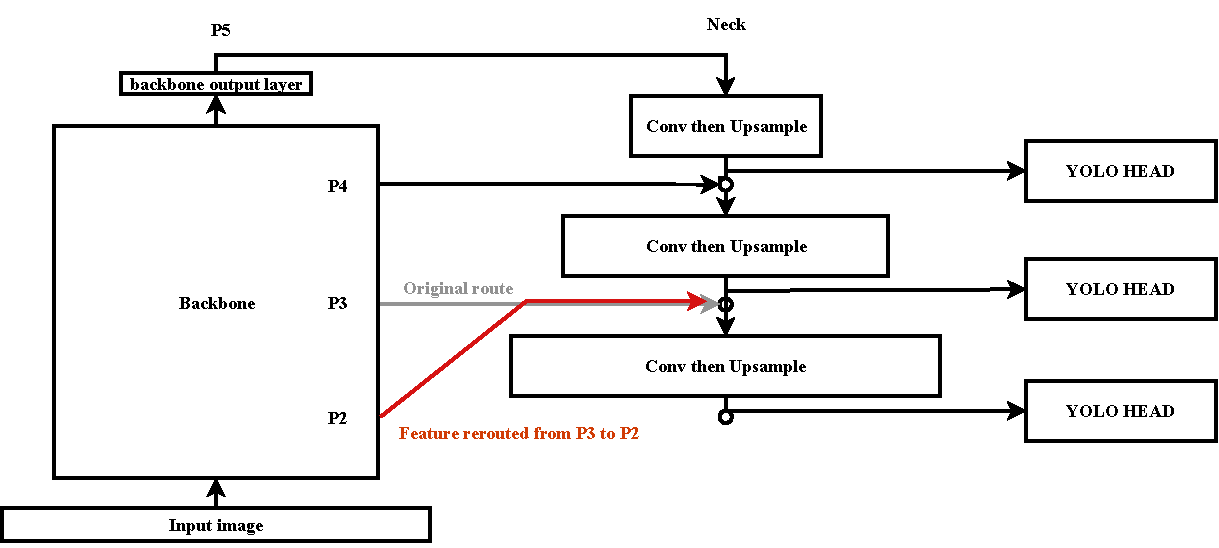
\includegraphics[width=0.4\textwidth]{../book/figures/neck-move-back.pdf}}
\caption{Rerouting Neck Feature-map Source}
\label{fig:neck-move-back}
\end{figure}
The source feature map that was fed on the feature pyramid can be rerouted 
to a shallower layer of the backbone (look at Fig. \ref{fig:neck-move-back}). 
By using the shallower layer, the input data will have a shorter propagation through the neural network.
This way, less information will be lost through propagation layer-by-layer.
%The shallower layer (layers that are closer to the input) has more 
%information about the image, albeit have less abstraction. 
%By doing this, we avoid the loss of information.

\subsubsection{Additional Detection Layer}
\begin{figure}[htbp]
\centerline{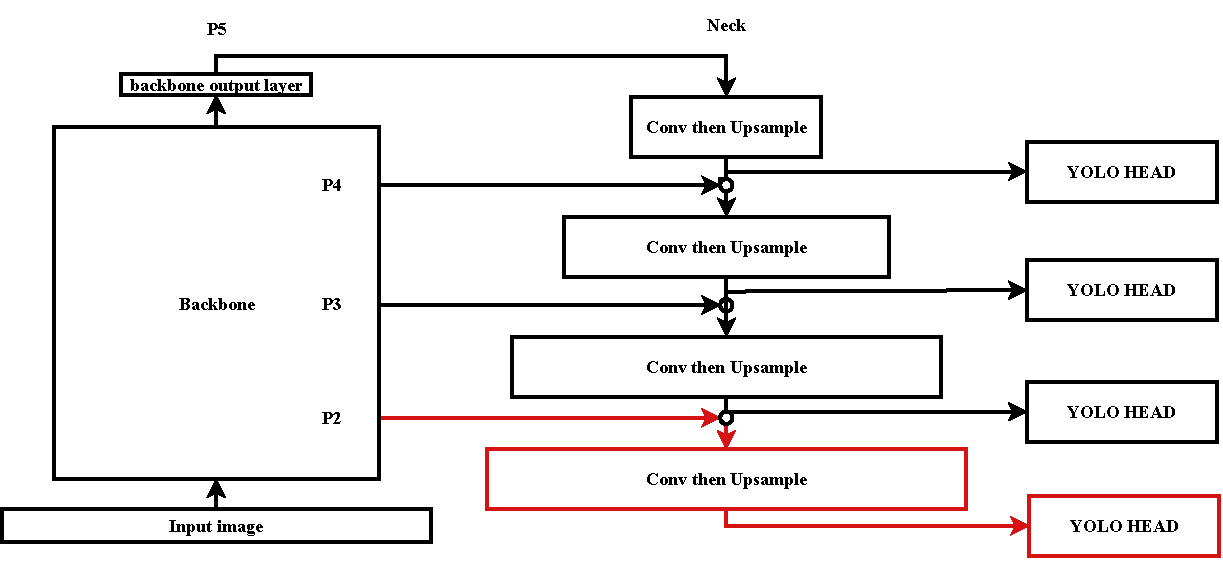
\includegraphics[width=0.4\textwidth]{../book/figures/addmorehead.pdf}}
\caption{Adding More Detection Layer}
\label{fig:add-head}
\end{figure}
An additional detection layer enable YOLOv7 to detect at more scales. With more scales,
the detection layers can be more specialized to specific cluster of data.
This approach has been tried in \cite{barunastra} by increasing the number of
detection layer from 2 to 3 in YOLOv4-tiny. In this experiment, we will increase
the number of detection layer from 3 to 4.
\subsubsection{Replacing Detection Layer to Decoupled Anchor-Free Head}
One of the advantage of anchor-free model to anchor-based model
is that it decreases the amount of heuristic tuning parameter as we don't
have to define the anchors. \cite{yolox}\cite{yolov6} reported that using anchor-free
head increases the accuracy and decreases the number of parameters in the model,
resulting in a faster and more accurate model.

\subsubsection{Partitioning Image for Inference}
Partitioning the image has the potential to improve the accuracy of small object detection.
By partitioning an image into multiple smaller images as shown in Fig. \ref{fig:partition}, 
the down-scaling factor of the original image to neural network input size is greatly reduced,
thereby reducing the loss of information. This approach allows the finer detail like small objects in the data.

One challenge with partitioning is the latency. As the neural network has to perform detection on each partition, the
total inference time is multiplied by the number of partitions.
\begin{figure}
  \centerline{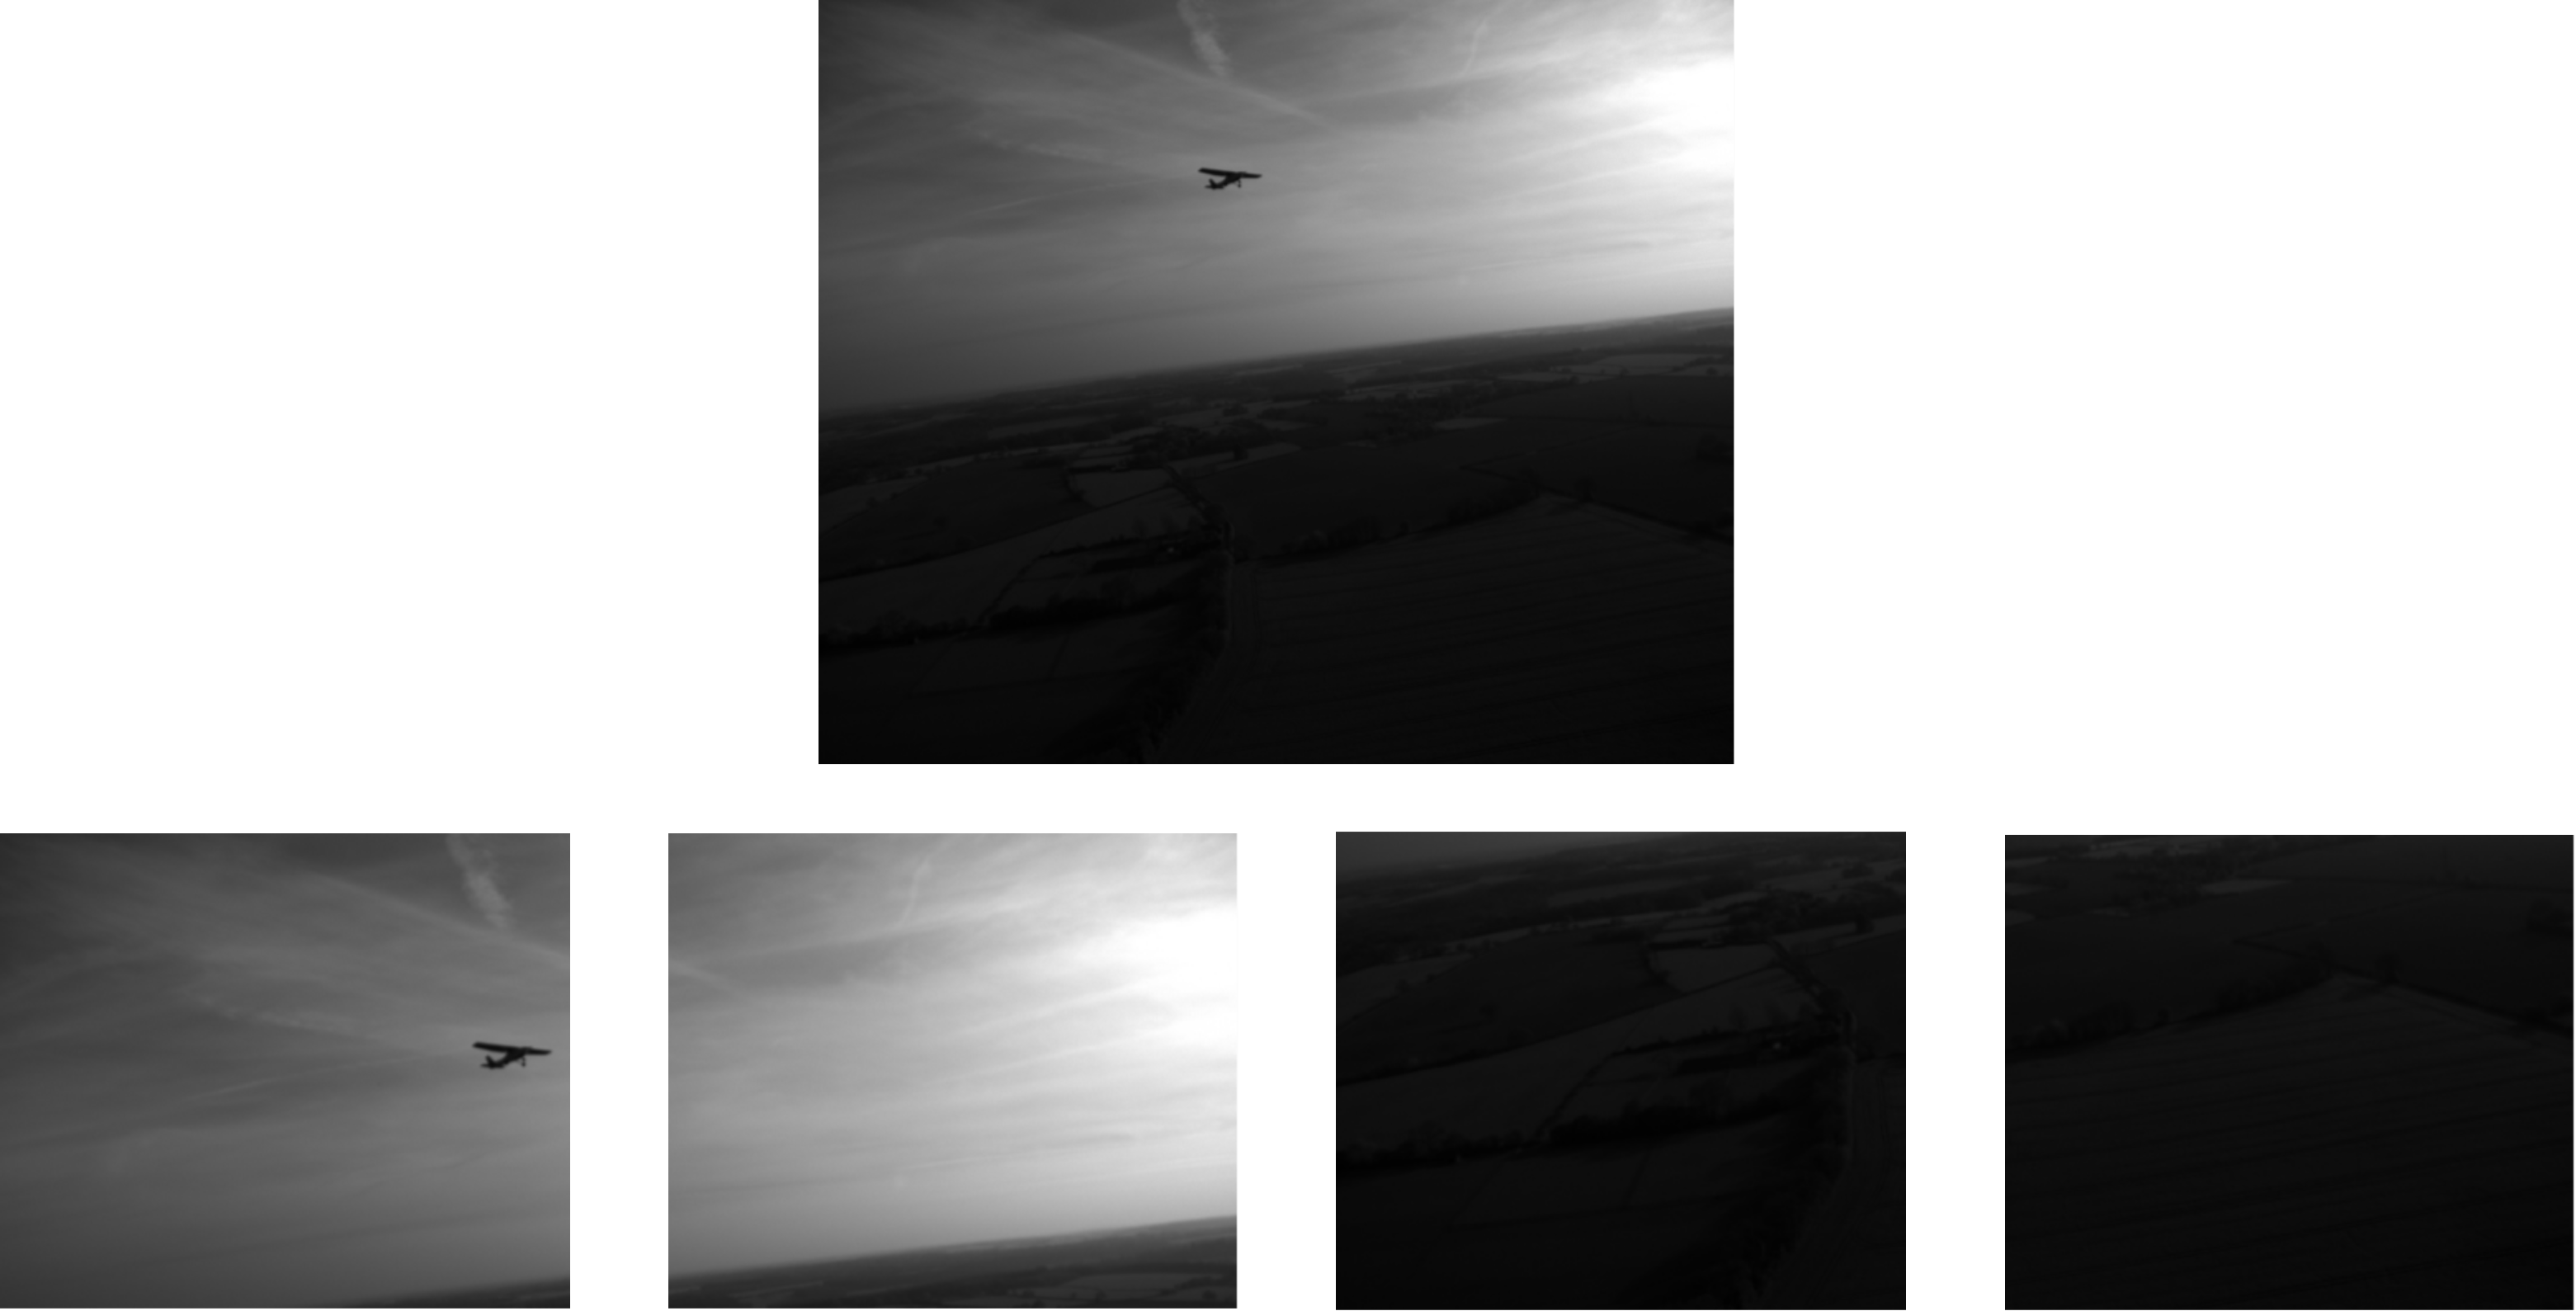
\includegraphics[width=\linewidth]{../book/figures/crop_strat.png}}
  \caption{Image Partitioning}
  \label{fig:partition}
\end{figure}

\section{Result}
\subsection{Initial Performance}
At first, we evaluate the performance of a plain YOLOv7 without all the
modifications proposed in section \ref{section:modifications}.
With 300 epochs and 400 data sample, we find the model was unable to detect
anything in the test set (mAP = 0).
For the purpose of comparison with other modification combination,
we will call this model as \verb*|YOLOv7-plain|.

\begin{figure*}
\centerline{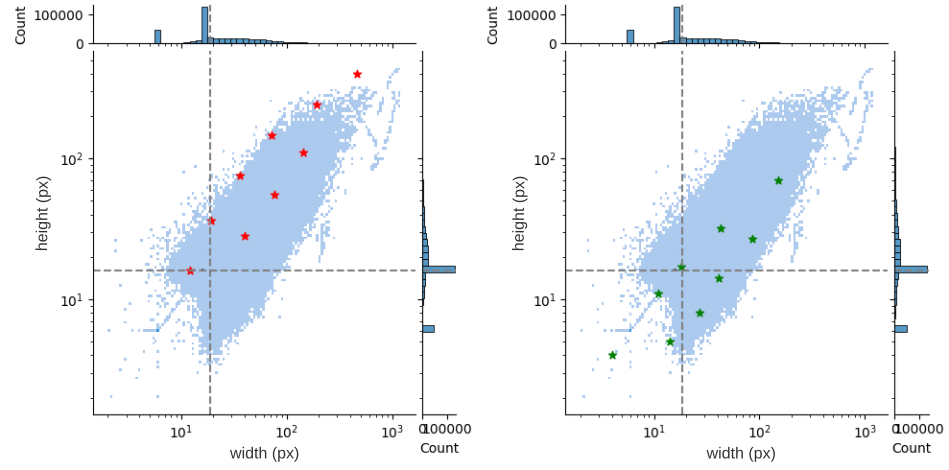
\includegraphics[width=0.9\textwidth]{../book/figures/anchor-dist-2.png}}
\caption{Anchor Points in Dataset Distribution. Left: Original Anchors. Right: Recalculated Anchors}
\label{fig:anchor-recalculated}
\end{figure*}

\subsection{Mosaic Augmentation and Anchor Recalculation}
In this section, we will compare 3 modification combination
\begin{itemize}
    \item YOLOv7-plain + Mosaic
    \item YOLOv7-plain + Anchor Recalculation
    \item YOLOv7-plain + Mosaic + Anchor Recalculation
\end{itemize}
We named these models as \verb|YOLOv7+M|, \verb|YOLOv7+AR|, and \verb|YOLOv7+MAR|.
We calculated the anchors using k-means clustering algorithm with log-distance function on the
training dataset. The result of the recalculation can be seen on Fig. \ref{fig:anchor-recalculated}.
As can be seen on the figure, 8 out of 9 of the old anchor points are placed in the first quadrant
of the median line. This means that those 8 anchors responsible only for 25\% of the dataset, which
is very ineffective. Compare that to the recalculated anchor. Every quadrant has at least one anchor
point responsible to it.
\begin{table}[htbp]
  \centering
  \caption{Mosaic Augmentation and Anchor Recalculation Performance}
  \label{tbl:mosaic_reanchor_performance}
  \vspace{-1ex}
    \begin{tabular}{ l l >{\hspace{4em}}c }
    \toprule[1.5pt]
    No & Model        &mAP@50 \\
    \midrule
    0  & \texttt{YOLOv7-plain}        & 0\%\\
    1  & \texttt{YOLOv7-M}            & 0\%\\
    2  & \texttt{YOLOv7-AR}           & 0\%\\
    3  & \texttt{\textbf{YOLOv7-MAR}} & \textbf{11.2}\%\\
    \midrule
       & Improvement                  & \textbf{\textcolor{green}{+11.2\%}}\\
    \bottomrule[1.5pt]
  \end{tabular}
\end{table}

Table \ref{tbl:mosaic_reanchor_performance} shows that the model was only able
to detect something on the test dataset after being applied both mosaic augmentation
and anchor recalculation.
For that reason, this model will be used as the basis for further 
modification, as it was the only model that could detect objects in test dataset.
Therefore, it should be assumed that the modification presented in
further sections is composed of mosaic augmentation and anchor recalculation, 
in addition to the respective modification that was applied, unless explicitly stated otherwise.

\subsection{EIoU Localization Loss}
In addition to just using EIoU, we also tested EIoU with its convexication technique 
mentioned in \cite{eiou}. The result can be seen on Table \ref{tbl:loss_function_perf}
It turns out that EIoU only worsen the performance of YOLOv7 in AOT dataset.
One possible reason for this is that: although CIoU have residue of regularization terms when the bounding boxes intersect,
these regularization helped the predicted box to fit faster. EIoU has a weaker values when the boxes not intersect.
Perhaps, on a longer training epoch, the EIoU can outperform CIoU.
\begin{table}[htbp]
  \centering
  \captionof{table}{EIoU Localization Loss Performance}
  \label{tbl:loss_function_perf}
  \vspace{-1ex}
    \begin{tabular}{ l l c }
    \toprule[1.5pt]
    No & Modification        &mAP@50 \\
    \midrule
    0  & \texttt{\textbf{YOLOv7-MAR +CIoU}} (original)     & \textbf{11.2}\%\\
    1  & \texttt{YOLOv7-MAR + EIoU}                & 0\%\\
    2  & \texttt{YOLOv7-MAR + EIoU + Convexication} & 4.92\%\\
    \midrule
       & Peningkatan                                & \textbf{\textcolor{red}{-6.28\%}}\\
    \bottomrule[1.5pt]
  \end{tabular}
\end{table}

\subsection{Rerouting Neck Feature-map Source}
\begin{figure}[htbp]
%\centerline{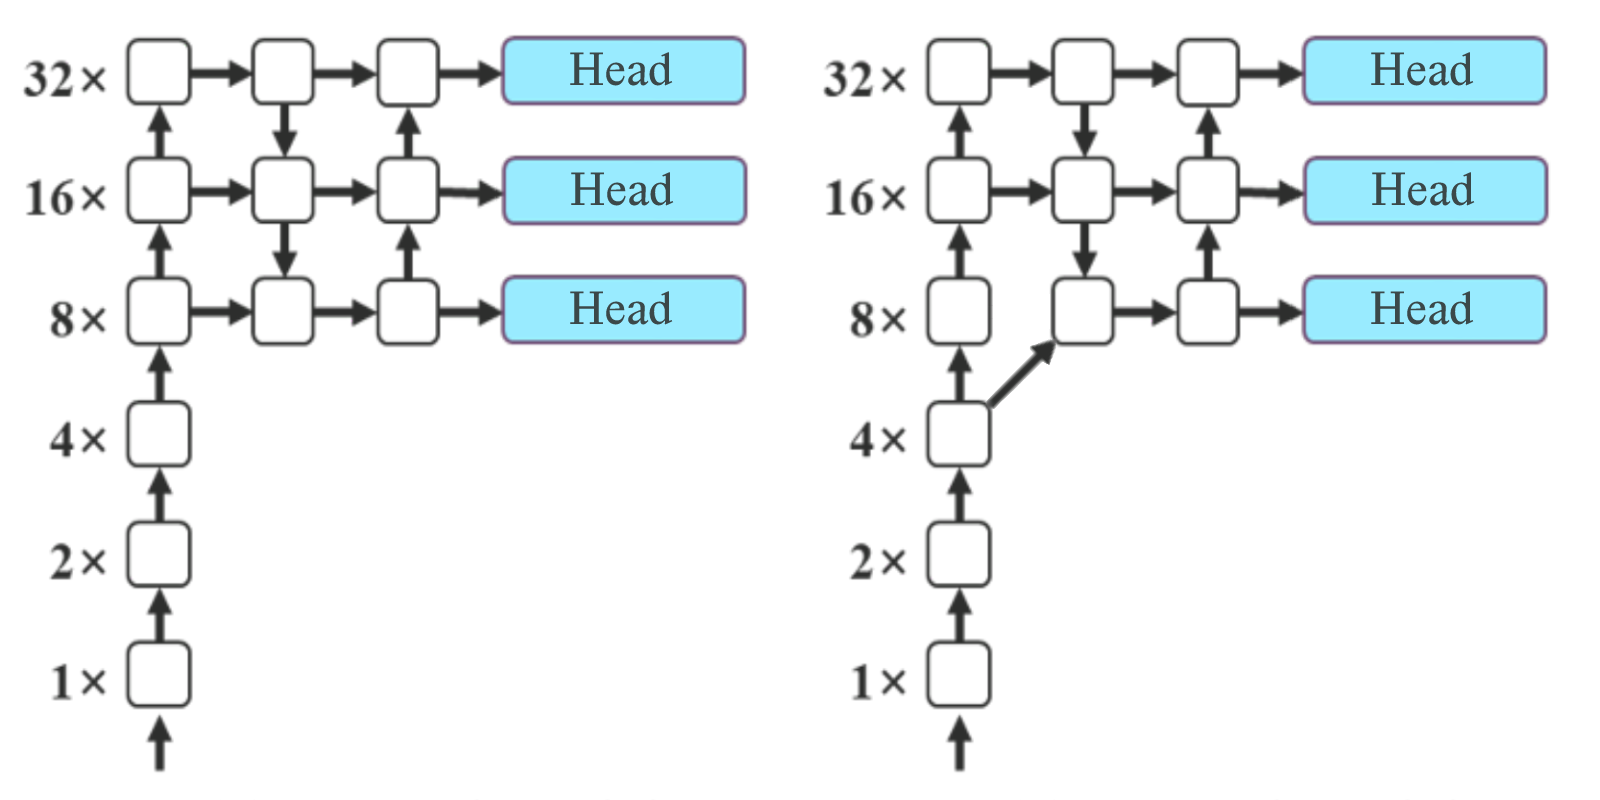
\includegraphics[width=0.5\textwidth]{../book/figures/deeperconn.png}}
  \begin{subfigure}[][][b]{0.5\linewidth}
    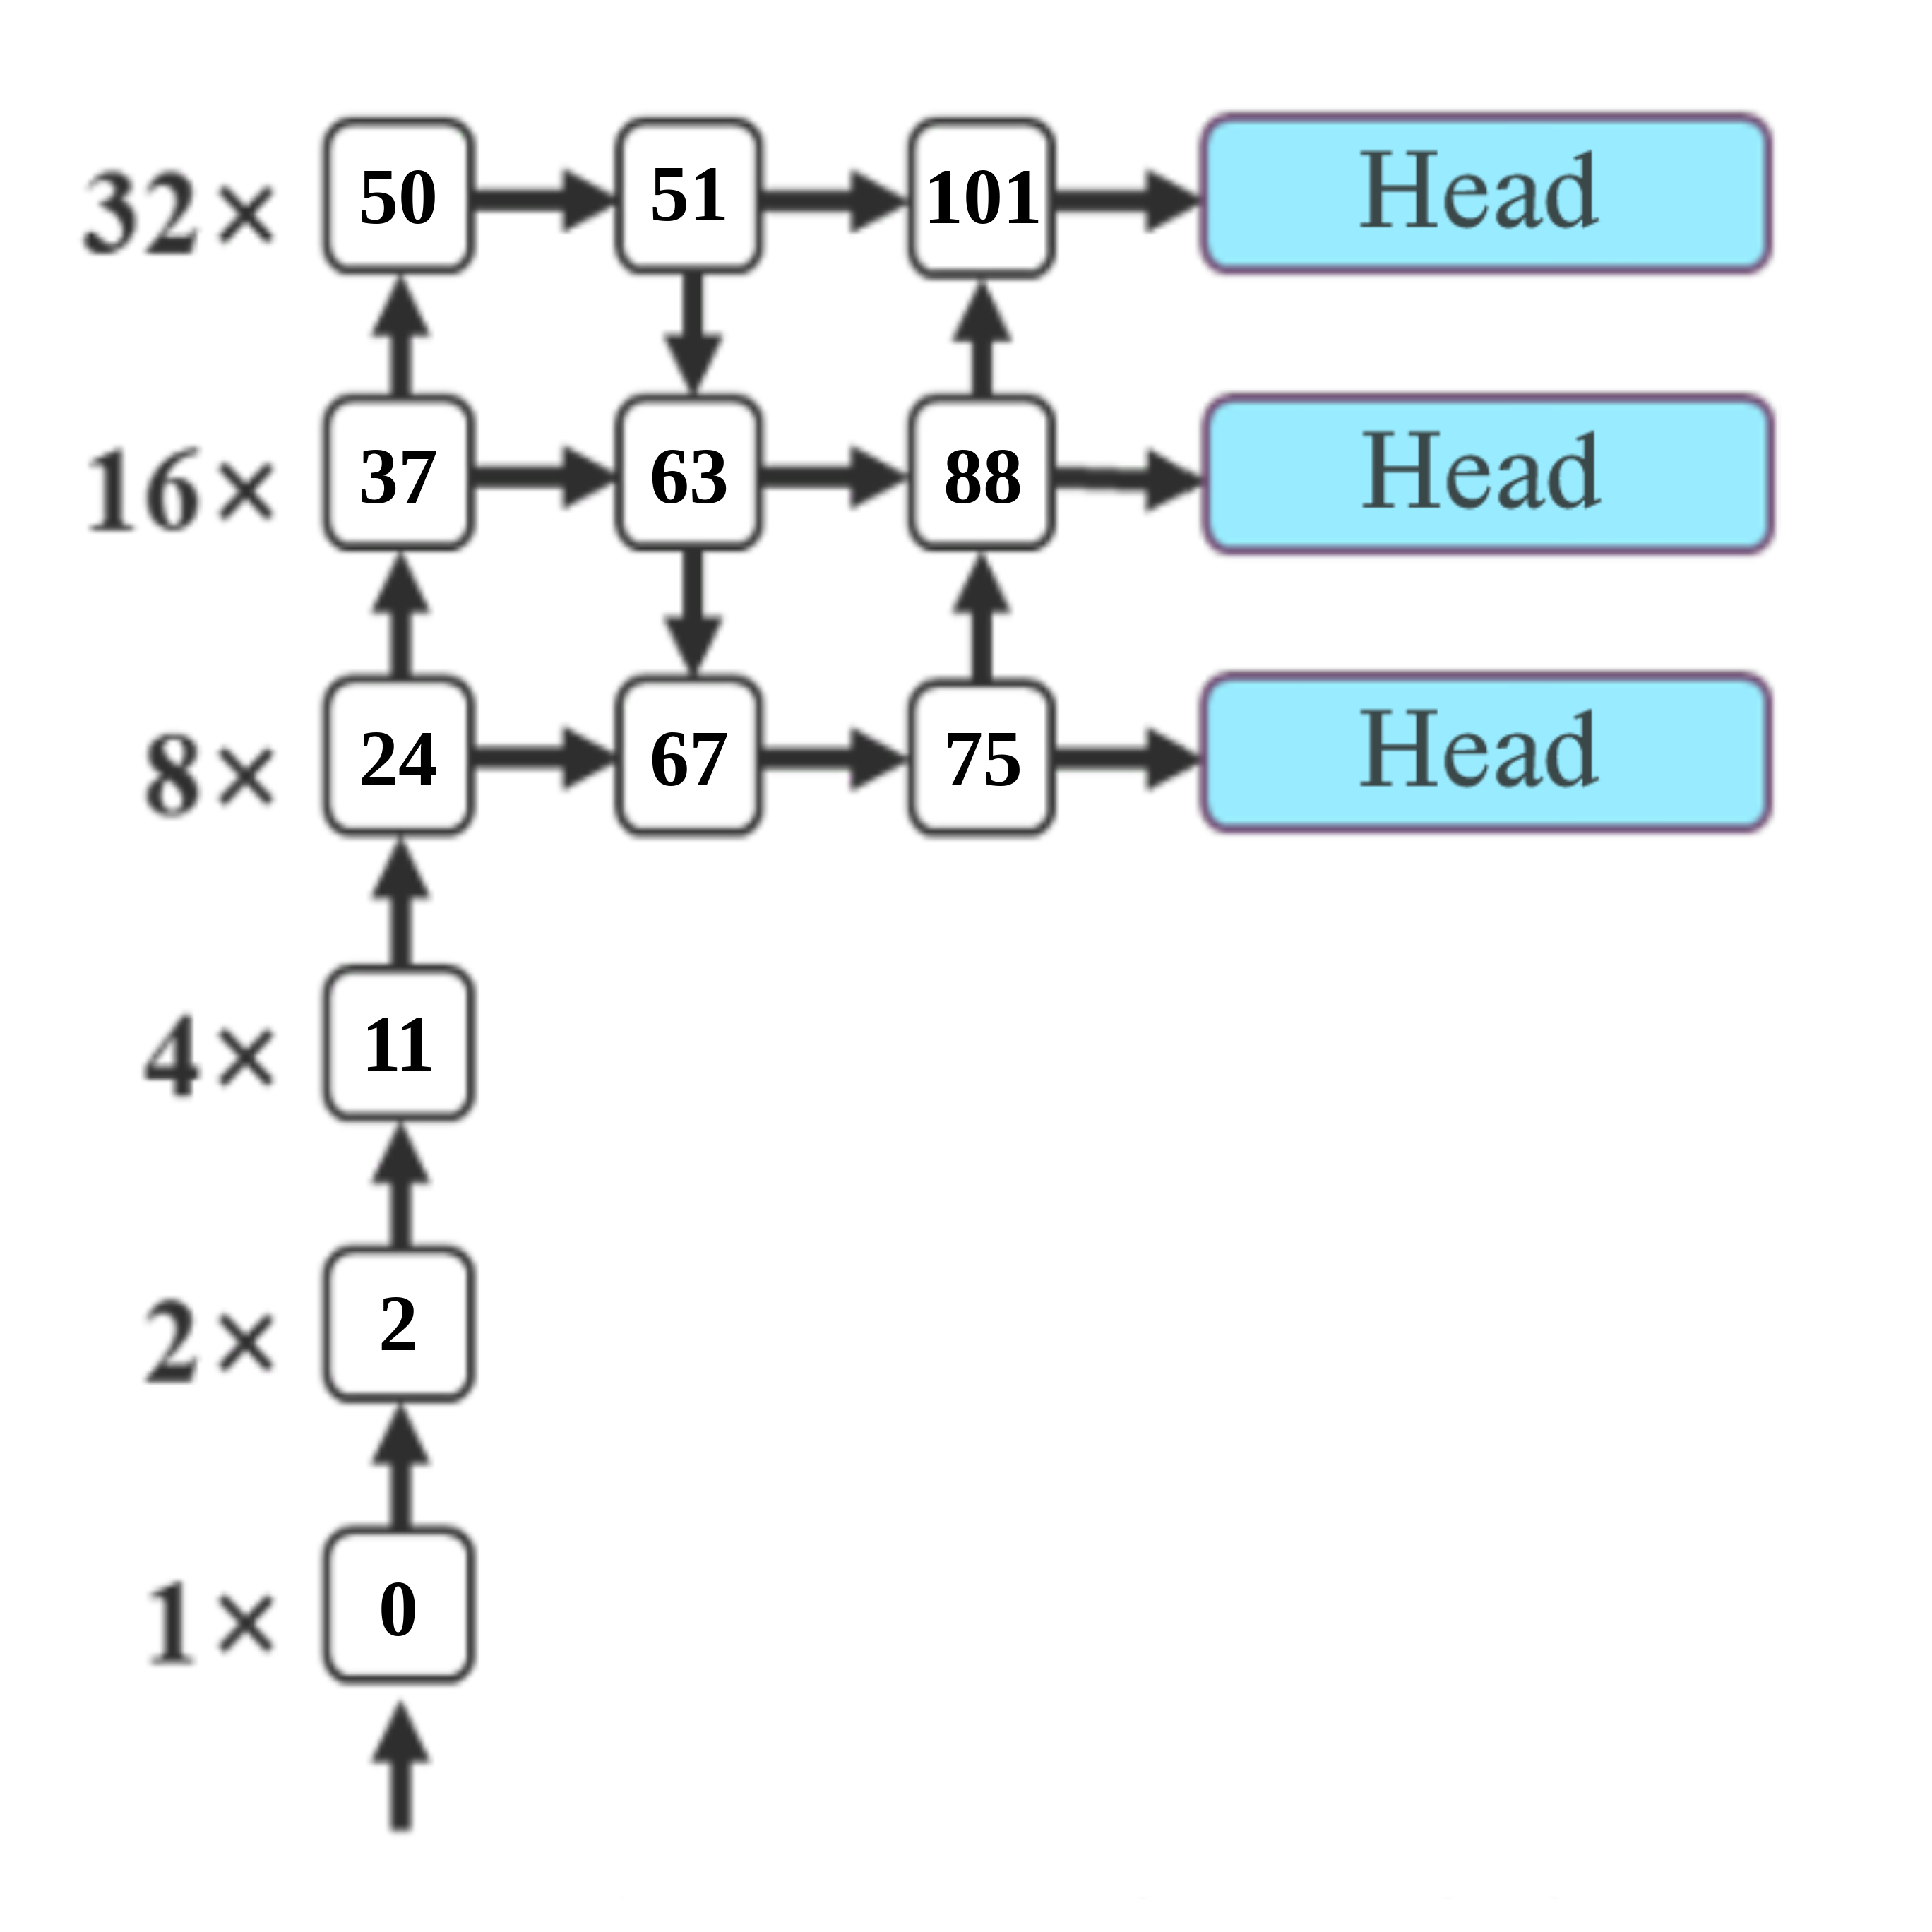
\includegraphics[width=1\linewidth]{../book/figures/deeperconn-before.png}
    \caption{Before Rerouting}
    \label{fig:deeperconn-before}
  \end{subfigure}\hfill%\hspace{4em}
  \begin{subfigure}[][][t]{0.5\linewidth}
    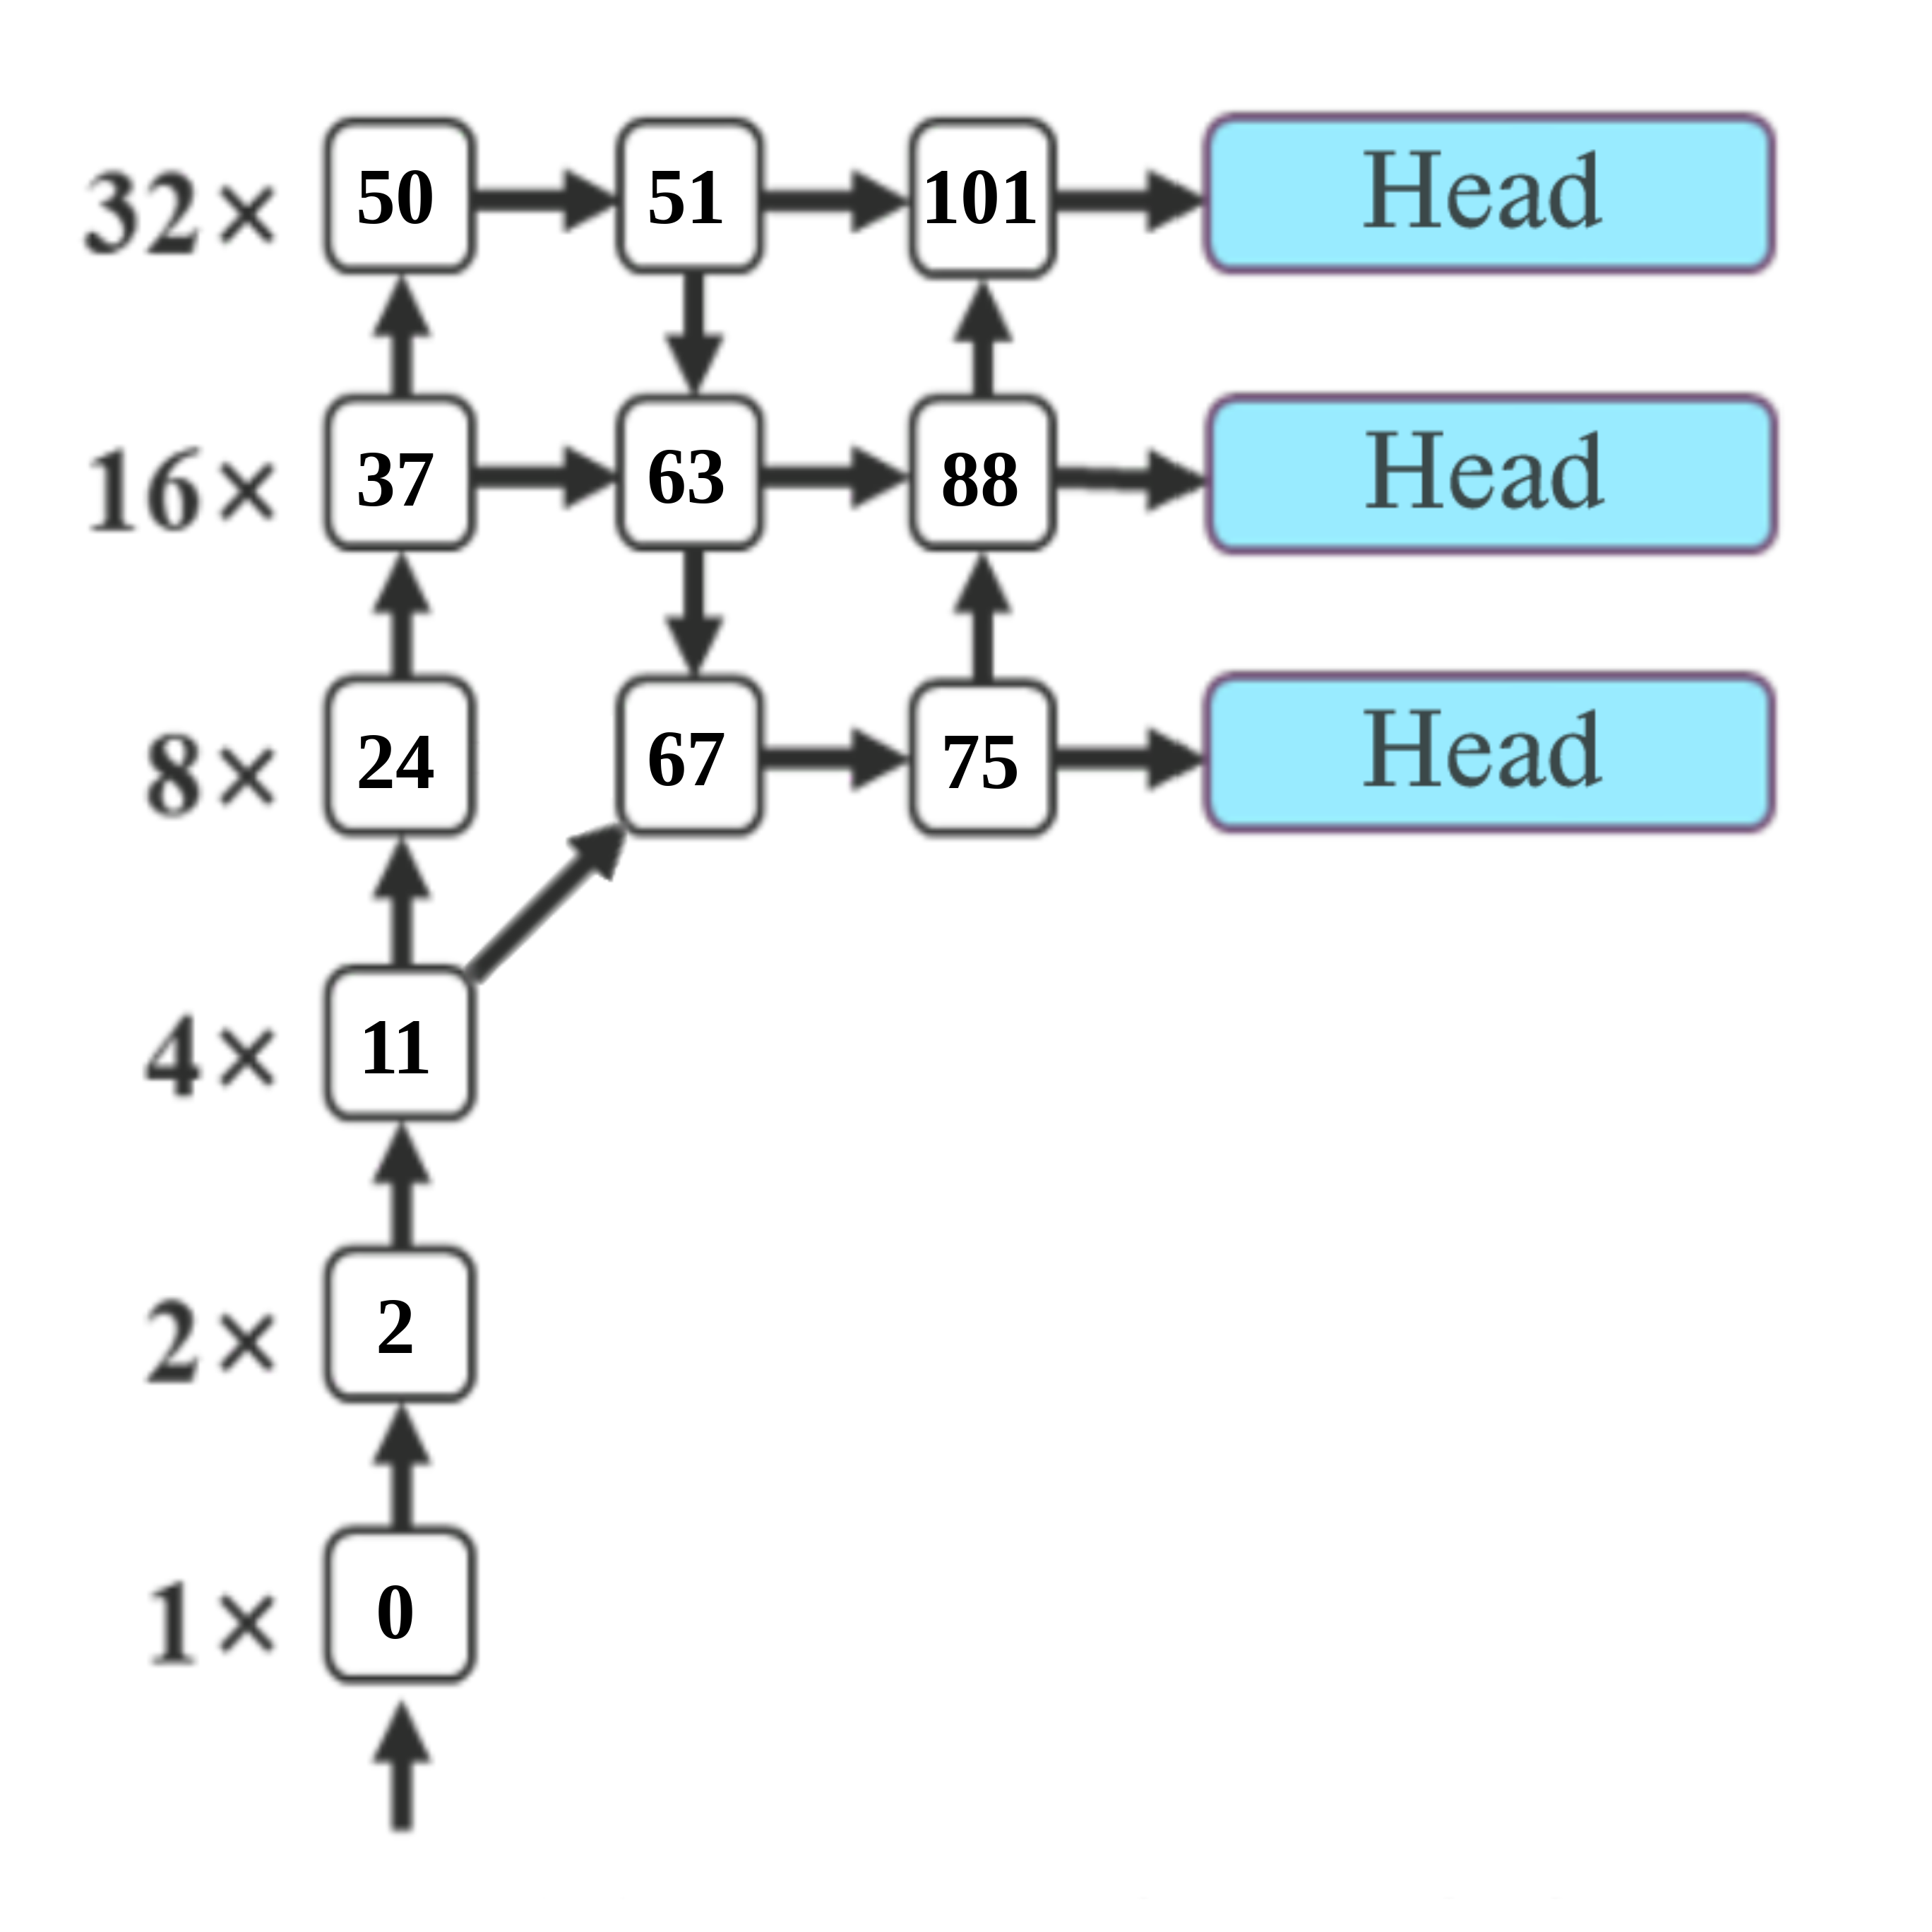
\includegraphics[width=1\linewidth]{../book/figures/deeperconn-after.png}
    \caption{After Rerouting}
    \label{fig:deeperconn-after}
  \end{subfigure}
\caption{Moving Feature-map Source}
\label{fig:deeperconn}
\end{figure}
We rerouted connection of the first pyramid from scale 8 to scale 4 of the backbone.
That is from layer 24 to layer 11 of the configuration file.
The moving of this connection is illustrated in Fig. \ref{fig:deeperconn}.
The performance of this modification can be seen on Table \ref{tbl:neck_backbone_perf}.
This modification managed to increase the mAP score by 2.98\%.

\begin{table}[htbp]
  \centering
  \caption{Rerouting Feature-map Source Performance}
  \label{tbl:neck_backbone_perf}
  \vspace{-1ex}
    \begin{tabular}{ l l c }
    \toprule[1.5pt]
    No & Modification                                      &mAP@50 \\
    \midrule
    0  & \texttt{YOLOv7-MAR}                           & 11.2\%\\
    1  & \texttt{\textbf{YOLOv7-MAR + rerouting}} & \textbf{14.09\%}\\
    \midrule
       & Improvement                                & \textbf{\textcolor{green}{+2.98\%}}\\
    \bottomrule[1.5pt]
  \end{tabular}
\end{table}


\subsection{Adding Extra Detection Layer}
\begin{figure}[htbp]
\centerline{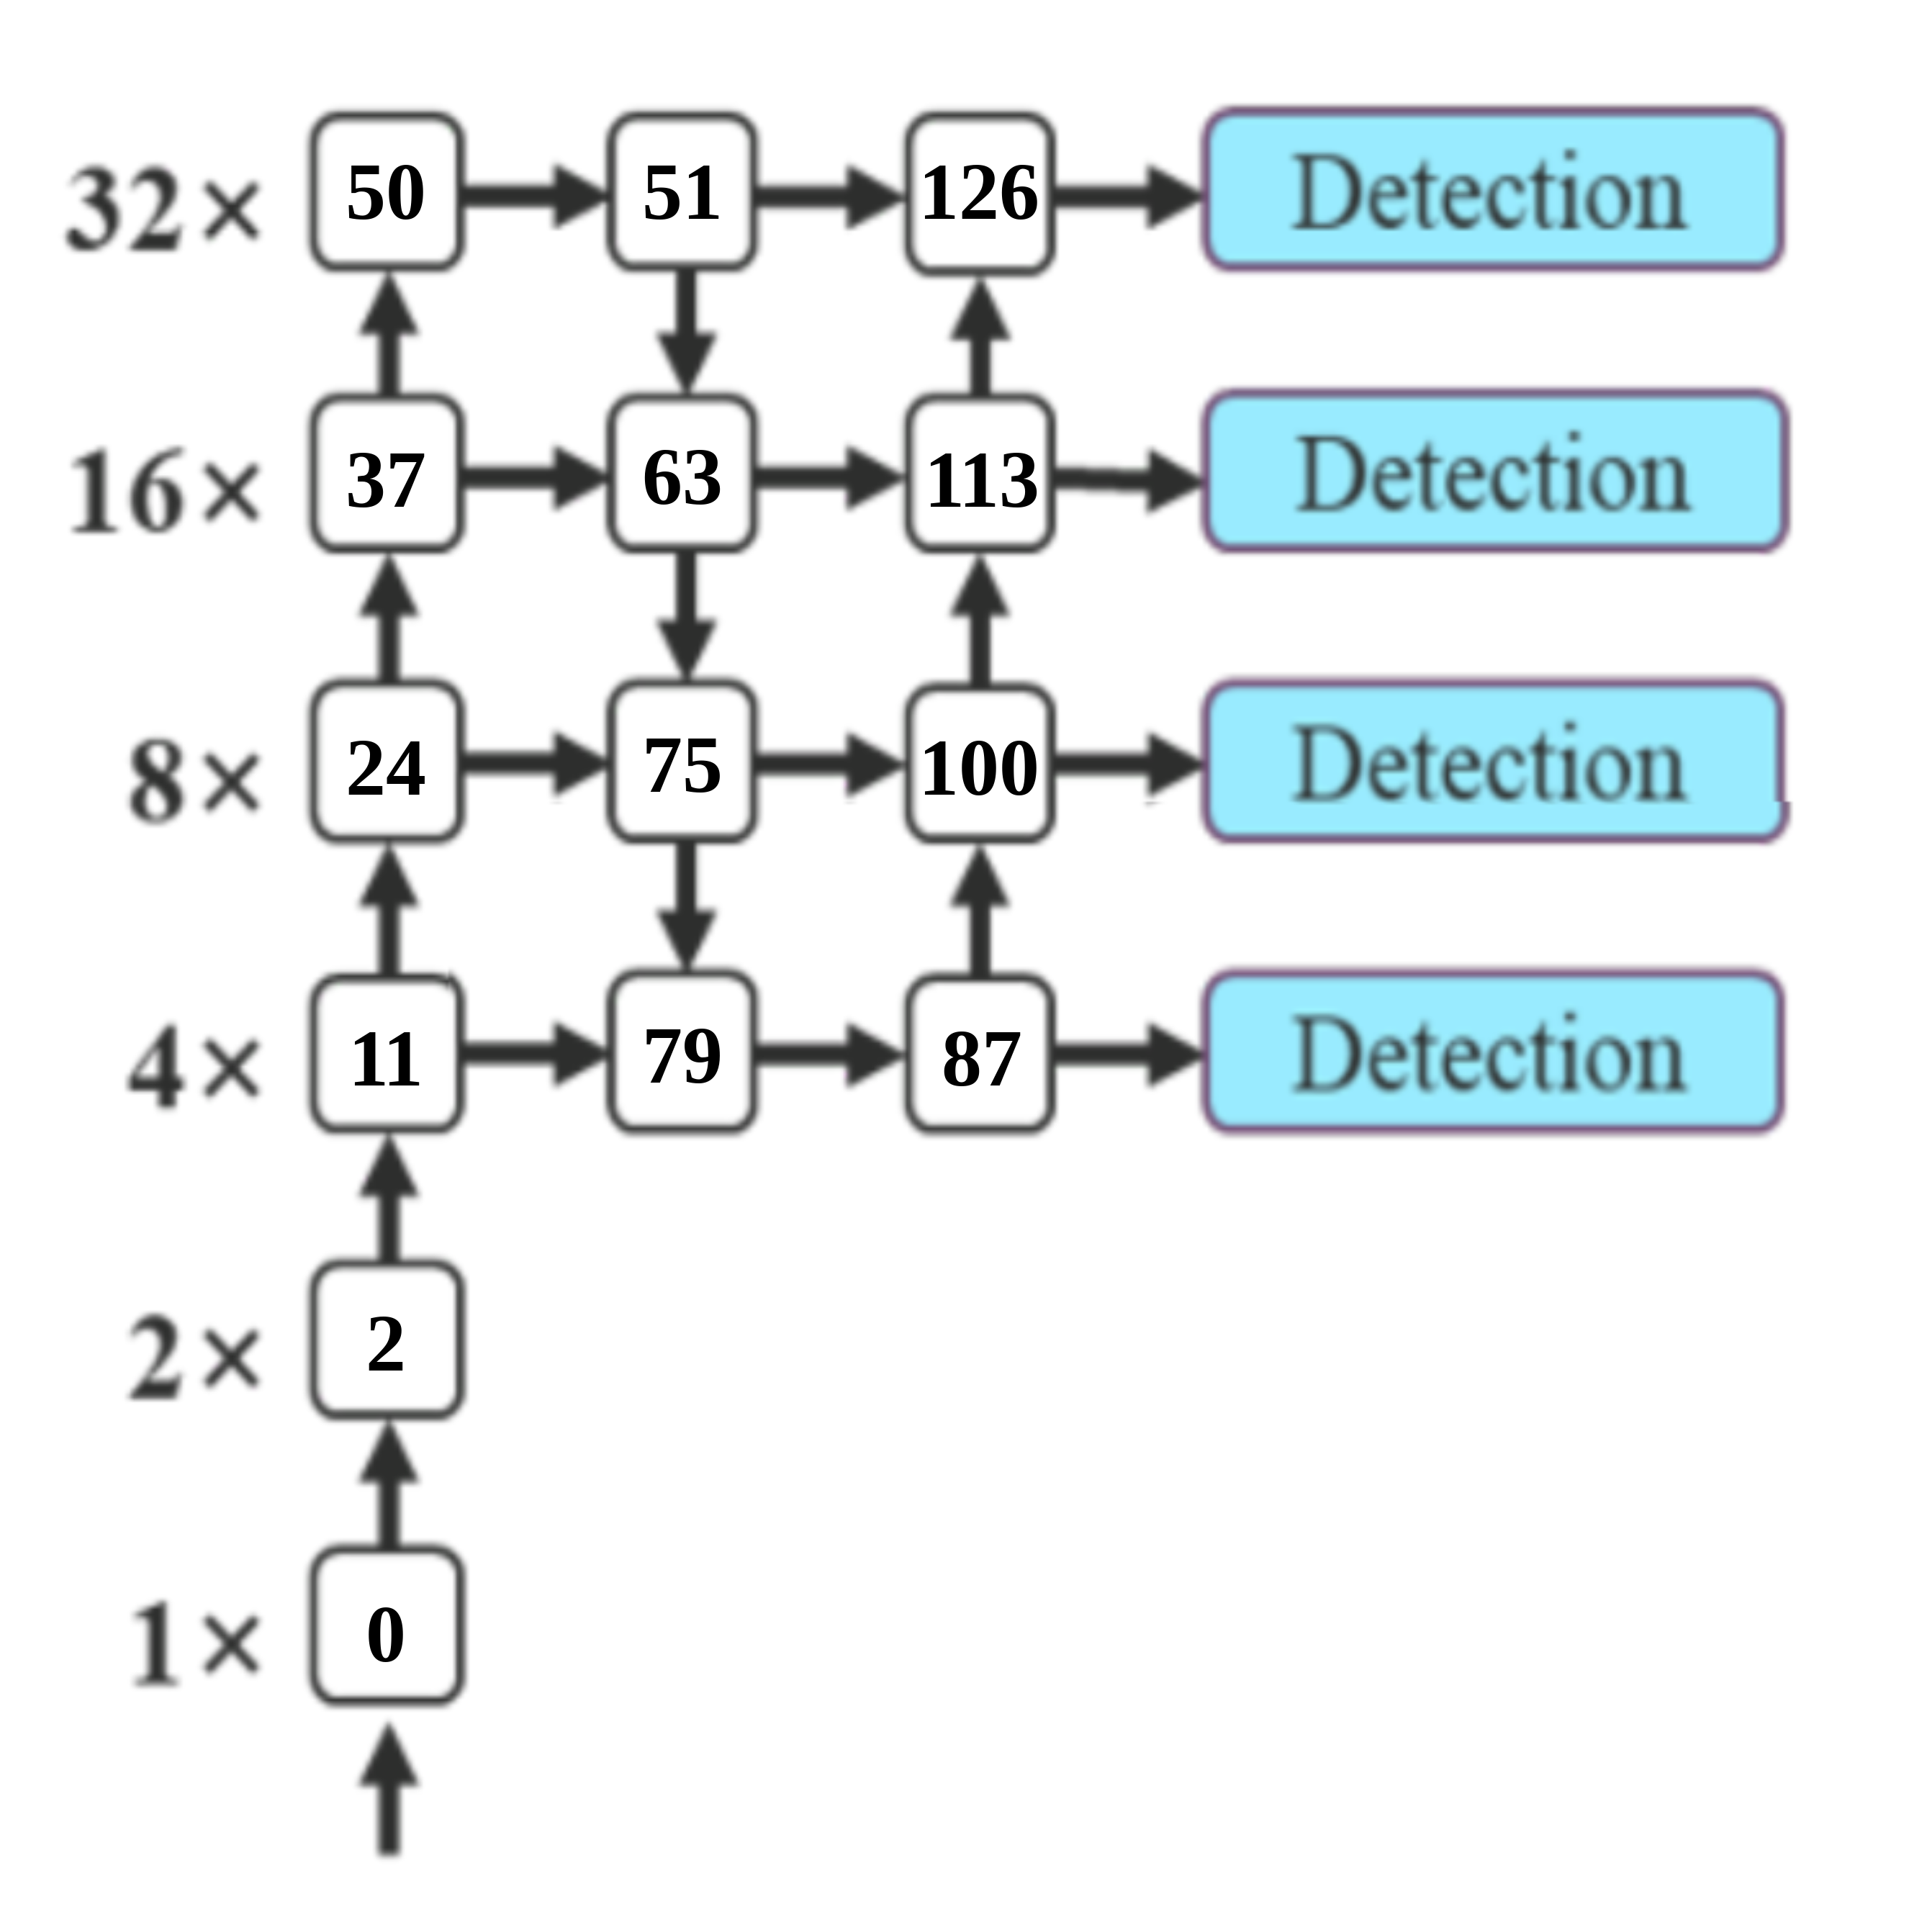
\includegraphics[width=0.3\textwidth]{../book/figures/addheadn.png}}
\caption{Adding More Detection Layer}
\label{fig:add-head-2}
\end{figure}
We add an extra feature pyramid stage connected to scale 4 of the backend, and put a detection head on it.
This modification is illustrated in Fig. \ref{fig:add-head-2}. We find that this modification
perform worse than rerouting as seen on Table \ref{tbl:addhead}.
\begin{table}[htbp]
  \centering
  \captionof{table}{Performance of Adding Extra Detection Layer}
  \label{tbl:addhead}
  \vspace{-1ex}
    \begin{tabular}{ l l c }
    \toprule[1.5pt]
    No & Modifikasi                                 &mAP@50 \\
    \midrule
    0  & \texttt{YOLOv7-MAR}                        & \textbf{11.2\%}\\
    1  & \texttt{YOLOv7-MAR + more head}            & 5.19\%\\
    \midrule
       & Improvement                                & \textbf{\textcolor{red}{-6\%}}\\
    \bottomrule[1.5pt]
  \end{tabular}
\end{table}

\subsection{Decoupled Anchor-free Head}
We changed the head of the model to anchor-free head with Task Aligned Labelling like in \cite{yolov6}.
After some fixing numerical instability due to division by very small object by clipping the values, we found a dramatic increase in mAP as seen on Table \ref{tbl:anchorfree}.
\begin{table}[htbp]
  \centering
  \captionof{table}{Anchor-free Head Performance}
  \label{tbl:anchorfree}
  \begin{adjustbox}{width=\linewidth}
  \begin{tabular}{ l l c }
  \toprule[1.5pt]
  No & Model                                 &mAP@50 \\
  \midrule
  0  & \texttt{YOLOv7-MAR (anchor head)}        & \textbf{11.2\%}\\
  1  & \texttt{YOLOv7-MAR + anchor-free head}       & 0\% Bug Fix Data Coming Up\\
  \bottomrule[1.5pt]
\end{tabular}
  \end{adjustbox}
  
\end{table}
\subsection{Image Partitioning}
We partitioned the images into 4 equal-sized images.
For training data, to reduce the number of negative samples that can impact the recall ability of the neural network,
we cropped the images in a way that the objects is within the cropping area for positive sample images and randomly cropping for negative sample images.
This cropping strategy was only done in the training set. For the test set, the cropping is done by dividing the image into four equal quadrants.

Since the partitioned image has smaller dimension, we experimented with smaller neural network input size.
The performance is shown on Table \ref{tbl:partition}. We can see that \texttt{YOLOv7+MAR + anchor-free} with input size 960 produced the greatest mAP score amongst other model when the images are partitioned into 4.

\begin{table}[htbp]
  \centering
  \captionof{table}{Modification Performance on Partitioned Images}
  \label{tbl:partition}
  \begin{tabular}{ l l c c c}
  \toprule[1.5pt]
  No & Model                                       &  Input Size  &Partition4 mAP@50               &mAP@50\\
  \midrule
  0  & \texttt{YOLOv7-AR}                          &     960      & 2.9\%                          &TBA\\
  1  & \texttt{YOLOv7-MAR}                         &     640      & 18.46\%                        &TBA\\
  3  & \texttt{YOLOv7-MAR}                         &     960      & 37.69\%                        &TBA\\
  4  & \texttt{YOLOv7-MAR + rerouting}             &     960      & 30.04\%                        &TBA\\
  5  & \texttt{YOLOv7-MAR + more head}             &     960      & 10.53\%                        &TBA\\
  6  & \texttt{YOLOv7-MAR + anchor-free}           &     640      & 37.57\%                        &TBA\\
  7  & \texttt{\textbf{YOLOv7-MAR + anchor-free}}  &     960      &\textbf{46.18\%}                &TBA\\
  %\midrule
  %   & Improvement                                 &              & \textbf{\textcolor{red}{-6\%}} &TBA\\
  \bottomrule[1.5pt]
\end{tabular}
\end{table}

\subsection{Latency}
Using Nvidia RTX 2080 Ti, we can obtain the speed of inference for each modification in Table \ref{tbl:latency}
We can see that every modified model can perform more than 10 inference per second.
Therefore, all the modifications can be considered for model selection.

As an additional information, the floating point operations for an inference of each models can be seen on table \ref{tbl:gflops}
\begin{table*}
  \centering
  \captionof{table}{Inference Speed of Modified Models}
  \label{tbl:latency}
  \begin{tabular}{ l l c c c}
  \toprule[1.5pt]
  No & Model                                       &   Input Size         &\multicolumn{2}{c}{Inference Speed}                   \\
     &                                             &                      &Not Reparameterized  &  Reparameterized   \\
  \midrule
  0  & \texttt{YOLOv7-MAR, plain, M, AR, EIoU}     &      1600            & 29.6 FPS            & TBA   \\
  1  & \texttt{YOLOv7-MAR + rerouting}             &      1600            & 23.28 FPS           & TBA   \\
  2  & \texttt{YOLOv7-MAR + more head}                 &      1600            & 15.91 FPS           & TBA   \\
  3  & \texttt{YOLOv7-MAR + anchor-free}               &      1600            & TBA                 & TBA   \\
  \midrule
  4  & \texttt{YOLOv7-MAR}                         &  Partition 4, 960    & TBA                 & TBA   \\
  5  & \texttt{YOLOv7-MAR + rerouting}             &  Partition 4, 960    & TBA                 & TBA   \\
  6  & \texttt{YOLOv7-MAR + more head}             &  Partition 4, 960    & TBA                 & TBA   \\
  7  & \texttt{YOLOv7-M + anchor-free}           &  Partition 4, 960    & TBA                 & TBA   \\
  \midrule
  8  & \texttt{YOLOv7-MAR}                         &  Partition 4, 640    & TBA                 & TBA   \\
  9  & \texttt{YOLOv7-MAR + rerouting}             &  Partition 4, 640    & TBA                 & TBA   \\
  10 & \texttt{YOLOv7-MAR + more head}             &  Partition 4, 640    & TBA                 & TBA   \\
  11 & \texttt{YOLOv7-M + anchor-free}           &  Partition 4, 640    & TBA                 & TBA   \\
  %\midrule
  %   & Improvement                                 &              & \textbf{\textcolor{red}{-6\%}} &TBA\\
  \bottomrule[1.5pt]
\end{tabular}
\end{table*}

\begin{table*}
  \centering
  \captionof{table}{FLOPs for Architectural Modifications with Different Input Sizes}
  \label{tbl:gflops}
  \begin{tabular}{ l l c c c}
  \toprule[1.5pt]
  No & Model                                       &   Input Size         & GFLOPs (\~MAC$\times$2)         \\
  \midrule
  0  & \texttt{YOLOv7-MAR, plain, M, AR, EIoU}     &      1600            & 552.11   \\ 
  1  & \texttt{YOLOv7-MAR + rerouting}             &      1600            & 692.02   \\
  2  & \texttt{YOLOv7-MAR + more head}             &      1600            & 627.25   \\
  3  & \texttt{YOLOv7-MAR + anchor-free}           &      1600            & 1374.47  \\ 
  \midrule
  4  & \texttt{YOLOv7-MAR, plain, M, AR, EIoU}     &      960             & 205.07  \\
  5  & \texttt{YOLOv7-MAR + rerouting}             &      960             & 257.03   \\
  6  & \texttt{YOLOv7-MAR + more head}             &      960             & 232.98    \\
  7  & \texttt{YOLOv7-M + anchor-free}             &      960             & 510.53  \\
  \midrule
  8  & \texttt{YOLOv7-MAR}                         &      640             & 89.39   \\
  9  & \texttt{YOLOv7-MAR + rerouting}             &      640             & 112.04   \\
  10 & \texttt{YOLOv7-MAR + more head}             &      640             & 101.55   \\
  11 & \texttt{YOLOv7-M + anchor-free}             &      640             & 222.53   \\
  %\midrule
  %   & Improvement                                 &              & \textbf{\textcolor{red}{-6\%}} &TBA\\
  \bottomrule[1.5pt]
\end{tabular}
\end{table*}
\section{Conclusion}
From the conducted experiment, we found that the best modification amongst the 
proposed modification candidates are the combination of mosaic augmentation, anchor-free head, and image partition.
The resulting modified model was able to produce mAP@50 score of 46.18\% on the test set while still able to
perform detection faster than 10 FPS on consumer GPU Nvidia RTX 2080 Ti.
%From the result of the experiment, we can conclude that, from the set of modification
%candidates proposed in this research, we found that the combination of mosaic augmentation,
%anchor recalculation, and modifying the connection of neck and backbone produces a model
%with the greatest mAP score which is 14.09\%.

\section{Discussion}
We have explored different ways to improve the detection of airborne objects in YOLOv7.
However, there are still more things we can try in the future to make it even better.
One idea is to use attention mechanisms, which help the model focus on important features related to airborne objects.
We could also investigate transfer learning and domain adaptation to leverage existing knowledge and adapt the model to specific situations.
Overall, there are still many opportunities for further research and enhancements in airborne object detection using YOLOv7.

%There are many more modifications that could be tried for this problem.
%For example, the uses of attention mechanism (\cite{attention}) have not been explored in this research.
%We will leave the experiment of these kinds of modification for future research.
%As of today, the modification proposed in this research only includes the modification that
%doesn't significantly impact the latency of the model. Some modification like partitioning
%the image and perform detection on each of partition could produce a great increase in mAP
%as the objects are magnified (number of partition) times. The latency also multiplied
%by the number of partition. But we can make the model faster by down-scaling the model.
%Thus, it is needed to find the optimal combination between down-scaling and number of partition
%that can produce a model that have high accuracy, but still have a latency that can be categorized
%as real-time.



%\begin{table}[htbp]
%\caption{Table Type Styles}
%\begin{center}
%\begin{tabular}{|c|c|c|c|}
%\hline
%\textbf{Table}&\multicolumn{3}{|c|}{\textbf{Table Column Head}} \\
%\cline{2-4} 
%\textbf{Head} & \textbf{\textit{Table column subhead}}& \textbf{\textit{Subhead}}& \textbf{\textit{Subhead}} \\
%\hline
%copy& More table copy$^{\mathrm{a}}$& &  \\
%\hline
%\multicolumn{4}{l}{$^{\mathrm{a}}$Sample of a Table footnote.}
%\end{tabular}
%\label{tab1}
%\end{center}
%\end{table}

%\begin{figure}[htbp]
%\centerline{\includegraphics{fig1.png}}
%\caption{Example of a figure caption.}
%\label{fig}
%\end{figure}

%Figure Labels: Use 8 point Times New Roman for Figure labels. Use words 
%rather than symbols or abbreviations when writing Figure axis labels to 
%avoid confusing the reader. As an example, write the quantity 
%``Magnetization'', or ``Magnetization, M'', not just ``M''. If including 
%units in the label, present them within parentheses. Do not label axes only 
%with units. In the example, write ``Magnetization (A/m)'' or ``Magnetization 
%\{A[m(1)]\}'', not just ``A/m''. Do not label axes with a ratio of 
%quantities and units. For example, write ``Temperature (K)'', not 
%``Temperature/K''.

%\section*{Acknowledgment}
%
%The preferred spelling of the word ``acknowledgment'' in America is without 
%an ``e'' after the ``g''. Avoid the stilted expression ``one of us (R. B. 
%G.) thanks $\ldots$''. Instead, try ``R. B. G. thanks$\ldots$''. Put sponsor 
%acknowledgments in the unnumbered footnote on the first page.

%\section*{References}

\bibliographystyle{IEEEtran}
\bibliography{../book/misc/bibliography.bib}

%\begin{thebibliography}{00}
%\bibitem{b1} G. Eason, B. Noble, and I. N. Sneddon, ``On certain integrals of Lipschitz-Hankel type involving products of Bessel functions,'' Phil. Trans. Roy. Soc. London, vol. A247, pp. 529--551, April 1955.
%\bibitem{b2} J. Clerk Maxwell, A Treatise on Electricity and Magnetism, 3rd ed., vol. 2. Oxford: Clarendon, 1892, pp.68--73.
%\bibitem{b3} I. S. Jacobs and C. P. Bean, ``Fine particles, thin films and exchange anisotropy,'' in Magnetism, vol. III, G. T. Rado and H. Suhl, Eds. New York: Academic, 1963, pp. 271--350.
%\bibitem{b4} K. Elissa, ``Title of paper if known,'' unpublished.
%\bibitem{b5} R. Nicole, ``Title of paper with only first word capitalized,'' J. Name Stand. Abbrev., in press.
%\bibitem{b6} Y. Yorozu, M. Hirano, K. Oka, and Y. Tagawa, ``Electron spectroscopy studies on magneto-optical media and plastic substrate interface,'' IEEE Transl. J. Magn. Japan, vol. 2, pp. 740--741, August 1987 [Digests 9th Annual Conf. Magnetics Japan, p. 301, 1982].
%\bibitem{b7} M. Young, The Technical Writer's Handbook. Mill Valley, CA: University Science, 1989.
%\end{thebibliography}
%\vspace{12pt}
%\color{red}
%IEEE conference templates contain guidance text for composing and formatting conference papers. Please ensure that all template text is removed from your conference paper prior to submission to the conference. Failure to remove the template text from your paper may result in your paper not being published.

\end{document}
